\documentclass[twoside]{article}
\usepackage{aistats2021}
\usepackage{amsmath, amsfonts, amsthm, amssymb}
\usepackage{graphicx}
\usepackage[colorlinks]{hyperref}
\usepackage[parfill]{parskip}
\usepackage{algpseudocode}
\usepackage{algorithm}
\usepackage{enumerate}
\usepackage[shortlabels]{enumitem}
\usepackage{mathtools}
\usepackage{tikz}
\usepackage{verbatim}

\usepackage{natbib}
\renewcommand{\bibname}{REFERENCES}
\renewcommand{\bibsection}{\subsubsection*{\bibname}}

\DeclareFontFamily{U}{mathx}{\hyphenchar\font45}
\DeclareFontShape{U}{mathx}{m}{n}{<-> mathx10}{}
\DeclareSymbolFont{mathx}{U}{mathx}{m}{n}
\DeclareMathAccent{\wb}{0}{mathx}{"73}

\DeclarePairedDelimiterX{\norm}[1]{\lVert}{\rVert}{#1}
\DeclarePairedDelimiterX{\seminorm}[1]{\lvert}{\rvert}{#1}

% Make a widecheck symbol (thanks, Stack Exchange!)
\DeclareFontFamily{U}{mathx}{\hyphenchar\font45}
\DeclareFontShape{U}{mathx}{m}{n}{
	<5> <6> <7> <8> <9> <10>
	<10.95> <12> <14.4> <17.28> <20.74> <24.88>
	mathx10
}{}
\DeclareSymbolFont{mathx}{U}{mathx}{m}{n}
\DeclareMathAccent{\wb}{0}{mathx}{"73}
% widecheck made

\newcommand{\eqdist}{\ensuremath{\stackrel{d}{=}}}
\newcommand{\Graph}{\mathcal{G}}
\newcommand{\Reals}{\mathbb{R}}
\newcommand{\iid}{\overset{\text{i.i.d}}{\sim}}
\newcommand{\convprob}{\overset{p}{\to}}
\newcommand{\convdist}{\overset{w}{\to}}
\newcommand{\Expect}[1]{\mathbb{E}\left[ #1 \right]}
\newcommand{\Risk}[2][P]{\mathcal{R}_{#1}\left[ #2 \right]}
\newcommand{\Prob}[1]{\mathbb{P}\left( #1 \right)}
\newcommand{\iset}{\mathbf{i}}
\newcommand{\jset}{\mathbf{j}}
\newcommand{\myexp}[1]{\exp \{ #1 \}}
\newcommand{\abs}[1]{\left \lvert #1 \right \rvert}
\newcommand{\restr}[2]{\ensuremath{\left.#1\right|_{#2}}}
\newcommand{\ext}[1]{\widetilde{#1}}
\newcommand{\set}[1]{\left\{#1\right\}}
\newcommand{\seq}[1]{\set{#1}_{n \in \N}}
\newcommand{\floor}[1]{\left\lfloor #1 \right\rfloor}
\newcommand{\Var}{\mathrm{Var}}
\newcommand{\Cov}{\mathrm{Cov}}
\newcommand{\diam}{\mathrm{diam}}

\newcommand{\emC}{C_n}
\newcommand{\emCpr}{C'_n}
\newcommand{\emCthick}{C^{\sigma}_n}
\newcommand{\emCprthick}{C'^{\sigma}_n}
\newcommand{\emS}{S^{\sigma}_n}
\newcommand{\estC}{\widehat{C}_n}
\newcommand{\hC}{\hat{C^{\sigma}_n}}
\newcommand{\vol}{\text{vol}}
\newcommand{\spansp}{\mathrm{span}~}
\newcommand{\1}{\mathbf{1}}

\newcommand{\Linv}{L^{\dagger}}
\DeclareMathOperator*{\argmin}{argmin}
\DeclareMathOperator*{\argmax}{argmax}

\newcommand{\emF}{\mathbb{F}_n}
\newcommand{\emG}{\mathbb{G}_n}
\newcommand{\emP}{\mathbb{P}_n}
\newcommand{\F}{\mathcal{F}}
\newcommand{\D}{\mathcal{D}}
\newcommand{\R}{\mathcal{R}}
\newcommand{\Rd}{\Reals^d}
\newcommand{\Nbb}{\mathbb{N}}

%%% Vectors
\newcommand{\thetast}{\theta^{\star}}
\newcommand{\betap}{\beta^{(p)}}
\newcommand{\betaq}{\beta^{(q)}}
\newcommand{\vardeltapq}{\varDelta^{(p,q)}}
\newcommand{\lambdavec}{\boldsymbol{\lambda}}

%%% Matrices
\newcommand{\X}{X} % no bold
\newcommand{\Y}{Y} % no bold
\newcommand{\Z}{Z} % no bold
\newcommand{\Lgrid}{L_{\grid}}
\newcommand{\Dgrid}{D_{\grid}}
\newcommand{\Linvgrid}{L_{\grid}^{\dagger}}
\newcommand{\Lap}{L}
\newcommand{\NLap}{{\bf N}}
\newcommand{\PLap}{{\bf P}}
\newcommand{\Id}{I}

%%% Sets and classes
\newcommand{\Xset}{\mathcal{X}}
\newcommand{\Vset}{\mathcal{V}}
\newcommand{\Sset}{\mathcal{S}}
\newcommand{\Hclass}{\mathcal{H}}
\newcommand{\Pclass}{\mathcal{P}}
\newcommand{\Leb}{L}
\newcommand{\mc}[1]{\mathcal{#1}}

%%% Distributions and related quantities
\newcommand{\Pbb}{\mathbb{P}}
\newcommand{\Ebb}{\mathbb{E}}
\newcommand{\Qbb}{\mathbb{Q}}
\newcommand{\Ibb}{\mathbb{I}}

%%% Operators
\newcommand{\Tadj}{T^{\star}}
\newcommand{\dive}{\mathrm{div}}
\newcommand{\dif}{\mathop{}\!\mathrm{d}}
\newcommand{\gradient}{\mathcal{D}}
\newcommand{\Hessian}{\mathcal{D}^2}
\newcommand{\dotp}[2]{\langle #1, #2 \rangle}
\newcommand{\Dotp}[2]{\Bigl\langle #1, #2 \Bigr\rangle}

%%% Misc
\newcommand{\grid}{\mathrm{grid}}
\newcommand{\critr}{R_n}
\newcommand{\dx}{\,dx}
\newcommand{\dy}{\,dy}
\newcommand{\dr}{\,dr}
\newcommand{\dxpr}{\,dx'}
\newcommand{\dypr}{\,dy'}
\newcommand{\wt}[1]{\widetilde{#1}}
\newcommand{\wh}[1]{\widehat{#1}}
\newcommand{\ol}[1]{\overline{#1}}
\newcommand{\spec}{\mathrm{spec}}
\newcommand{\LE}{\mathrm{LE}}
\newcommand{\LS}{\mathrm{LS}}
\newcommand{\SM}{\mathrm{SM}}
\newcommand{\OS}{\mathrm{OS}}
\newcommand{\PLS}{\mathrm{PLS}}

%%% Order of magnitude
\newcommand{\soom}{\sim}

%%% Theorem environments
\newtheorem{theorem}{Theorem}
\newtheorem{conjecture}{Conjecture}
\newtheorem{lemma}{Lemma}
\newtheorem{example}{Example}
\newtheorem{corollary}{Corollary}
\newtheorem{proposition}{Proposition}
\newtheorem{assumption}{Assumption}
\newtheorem{remark}{Remark}


\theoremstyle{definition}
\newtheorem{definition}{Definition}[section]

\theoremstyle{remark}


\begin{document}
	
\twocolumn[

	\aistatstitle{Minimax optimal Laplacian smoothing}
	
	\aistatsauthor{Alden Green, Sivaraman Balakrishnan, and Ryan J. Tibshirani}

	\aistatsaddress{Carnegie Mellon University}]
	

\begin{abstract}
	In this paper we study the statistical properties of Laplacian smoothing, a graph-based approach to non-parametric regression. Under standard regularity conditions, we establish upper bounds on the error of the Laplacian smoothing estimator $\wh{f}$, and a goodness-of-fit test based on $\wh{f}$. These upper bounds match the minimax optimal estimation and testing rates of convergence over the first-order Sobolev class $H^1(\Xset)$, where $\Xset \subset \Rd$ and $1 \leq d < 4$; in the estimation problem, they are within a $\log n$ factor of optimal when $d = 4$. Additionally, we prove that Laplacian smoothing is manifold adaptive: if $\Xset$ is an $m$ dimensional manifold embedded in $\Reals^d$ with $m \ll d$, then the error rate of Laplacian smoothing methods depends only on the intrinsic dimension $m$ and not on the ambient dimension $d$. Empirically, we show that Laplacian smoothing appears not to be minimax optimal over $H^1(\Xset)$ when $d > 4$. 
\end{abstract}

\section{INTRODUCTION}
In the nonparametric regression problem, we observe samples $(X_1,Y_1),\ldots,(X_n,Y_n)$ according to the signal plus noise model
\begin{equation}
\label{eqn:signal_plus_noise_model}
Y_i = f_{0}(X_i) + \varepsilon_i,
\end{equation}
with $\varepsilon_i \sim N(0,1)$ independent Gaussian noise. Our goal is to perform statistical inference on the unknown regression function $f_0$, by which we mean either \emph{estimating} $f_0$ or more simply \emph{testing} whether $f_0 = 0$, i.e whether there is any signal present. 

The Laplacian smoothing estimator $\wh{f}$ \citep{smola2003} is a penalized least squares estimator. It is defined with respect to the weighted graph $G = \bigl(\{1,\ldots,n\},W\bigr)$ over the vertices $\{1,\ldots,n\}$ (equivalently, over the design points $X_1,\ldots,X_n$) as
\begin{equation}
\label{eqn:laplacian_smoothing}
\wh{f} :=  \min_{f \in \Reals^n} \biggl\{\sum_{i = 1}^{n}(Y_i - f_i)^2 + \rho \cdot f^T \Lap f \biggr\}.
\end{equation}
Here $\Lap$ is the graph Laplacian matrix (defined in Section~\ref{sec:problem_setup_and_background}), and the penalty
\begin{equation*}
f^T \Lap f = \frac{1}{2} \sum_{i,j = 1}^{n} W_{ij}\bigl(Y_i - Y_j\bigr)^2
\end{equation*}
encourages $\wh{f}_i \approx \wh{f}_j$ when $W_{ij}$ is large. Assuming~\eqref{eqn:laplacian_smoothing} is a reasonable estimator of $f_0$, the squared empirical norm
\begin{equation}
\label{eqn:laplacian_smoothing_test}
\wh{T} := \frac{1}{n}\bigl\|\wh{f}\bigr\|_2^2 
\end{equation}
is in turn a reasonable statistic to assess whether or not $f_0 = 0$. 

Of course there exist many methods for nonparametric regression \citep{gyorfi2006,wasserman2006,tsybakov2008_book}, but Laplacian smoothing has its own set of advantages. For instance:
\begin{itemize}
	\item \emph{Computational ease.} Laplacian smoothing is fast, easy, and stable to compute. The estimate $\wh{f}$ can be computed by solving a symmetric, diagonally dominant linear system. There are known extremely fast and reliable solvers for exactly this problem (see e.g. the seminal papers of \cite{spielman2011,spielman2013,spielman2014}, or the monograph by~\cite{vishnoi2012} and references therein).
	\item \emph{Generality.} Laplacian smoothing is well defined whenever one can associate a graph with some observed responses. This generality lends itself to many different data modalities: for instance text and image classification, to name only two \citep{kondor2002, belkin03a,belkin2006}. 
	\item \emph{Weak supervision.} Although we study Laplacian smoothing in the supervised learning setup~\eqref{eqn:signal_plus_noise_model}, it can be easily adapted to the semi-supervised or unsupervised settings \citep{nadler09,slepcev17,dunlop2020,calder2019b}.
\end{itemize}

For these reasons, a body of work has emerged analyzing the statistical properties of Laplacian smoothing, and graph-based methods more generally. Roughly speaking, these works can be divided into two categories, based on the perspective they adopt. 
\begin{itemize}
	\item In the \emph{discrete (fixed design) perspective}, the design points $\{X_1,\ldots,X_n\}$ and the graph $G$ are treated as fixed, and inference is carried out on the evaluations $\bigl(f_0(X_1),\ldots,f_0(X_n)\bigr) \in \Reals^n$. In this context, tight upper bounds have been derived on the error of graph-based estimators \citep{wang2016, sadhanala16,sadhanala17,kirichenko2017,kirichenko2018} and tests \citep{sharpnack2013,sharpnack2013b,sharpnack2015}, which certify that such procedures are \emph{optimal} over ``function'' classes $\mc{F} \subseteq \Reals^n$. The downside of this work is that, depending on the context, it may be unnatural to assume a priori that the graph $G$ is fixed, or that the evaluations $\bigl(f_0(X_1),\ldots,f_0(X_n)\bigr)$ belongs to some discrete ``function'' class.
	\item In the arguably more natural \emph{continuum (random design) perspective},  one assumes the design points $\{X_1,\ldots,X_n\}$ are sampled independently from some distribution $P$ supported on a domain $\Xset$. Inference is drawn on the regression function $f_0: \Xset \to \Reals$, which is assumed to be smooth in some sense, e.g. it possesses a first derivative bounded in $L^{\infty}$ (Holder) or $\Leb^2$ (Sobolev) norm.
	
	To conduct graph-based inference on $f_0$, the user builds a neighborhood graph over the design points, so that $W_{ij}$ is large iff $X_i$ and $X_j$ are close, say in Euclidean distance, and then solves e.g.~\eqref{eqn:laplacian_smoothing} or~\eqref{eqn:laplacian_smoothing_test}. In this context, various graph-based procedures have been shown to be \emph{consistent}: as $n \to \infty$, they converge to a \emph{continuum} limit (see \citep{belkin07,trillos2018,vonluxburg2008} among others). However, until recently such statements were not accompanied by error rates, and such error rates as have been proved \citep{lee2016,trillos2020} are not optimal over continuum function spaces, such as H\"{o}lder or Sobolev classes. 
\end{itemize}
Viewed as a whole, this body of work leaves a key question unanswered: 

\begin{quote}{What are the optimality properties of graph Laplacian smoothing, viewed as an estimator of a function $f_0$ that is smooth in a continuum sense?} 
\end{quote}
On the one hand, this is no small question---rather, it is arguably the fundamental question of nonparametric regression, and without an answer one cannot fully compare the statistical properties of Laplacian smoothing to its competitors. On the other hand, it seems difficult to answer: there is a fundamental gap between the \emph{discrete} smoothness imposed by the penalty $f^T \Lap f$ in~\eqref{eqn:laplacian_smoothing} and the \emph{continuum} smoothness assumed on $f_0$, and to obtain sharp upper bounds we needs to bridge this gap in a suitably tight sense.

\section{SUMMARY OF RESULTS}
In light of this last point, it is worth stepping back for a moment and asking: do we really need to a solve a discrete problem at all? After all, we could have instead directly leveraged the (continuum) smoothness of $f_0$ by solving the following variational problem:
\begin{equation}
\label{eqn:thin_plate_spline}
\wt{f} := \argmin_{f} \biggl\{\sum_{i = 1}^{n} \bigl(Y_i - f(X_i)\bigr)^2 + \rho \cdot \int_{\Xset} \|\nabla f(x)\|^2 \,dx \biggr\}
\end{equation}

\begin{itemize}
	\item 
	Of course, there are computational advantages to Laplacian smoothing, as mentioned previously, but let's leave those aside for the second, and ask only whether there is any statistical advantage.
	\item At first blush, the more likely answer is no. As we detail in Section~\ref{sec:minimax_optimal_laplacian_smoothing}, the Laplacian smoothing problem~\eqref{eqn:laplacian_smoothing} and variational problem~\eqref{eqn:thin_plate_spline} are in fact intimately connected; indeed~\eqref{eqn:laplacian_smoothing} can be viewed as a discrete and noisy approximation to~\eqref{eqn:thin_plate_spline}. At first blush, this suggests that Laplacian smoothing should at best of inherent the statistical properties thin-plate splines, and at worst possibly have meaningfully larger error.
	\item However the actual story is quite different: remarkably, Laplacian smoothing outperforms smoothing splines! 
	\item Laplacian smoothing also demonstrates manifold 
\end{itemize}

\paragraph{Future extensions.}






Our work addresses this gap, and our main contributions can all be summarized as follows: Laplacian smoothing over a random design is minimax optimal over certain first-order \emph{continuum} Sobolev balls. We will show that this is true for the estimator $\wh{f}$ and test statistic $\wh{T}$, when $\Xset \subset \Rd$ is a full-dimensional domain and $1 \leq d \leq 4$. Additionally, we will consider the \emph{manifold hypothesis}---roughly, that $\Xset$ is a manifold embedded in $\Rd$, with intrinsic dimension $m \ll d$---and derive upper bounds which depend only on the intrinsic dimension $m$, and are independent of the ambient dimension $d$; these bounds too will be optimal. For ease of reading, we provide the upper bounds derived in all our main theorems in Table~\textcolor{red}{(1)}.

\begin{table}
\begin{center}
\begin{tabular}{p{.1\textwidth} | p{.14\textwidth} p{.12\textwidth} }
	Dimension & Laplacian smoothing \eqref{eqn:laplacian_smoothing} & Thin-plate splines \eqref{eqn:thin_plate_spline} \\
	\hline
	$d = 1$ & $n^{-2/3}$ & \textcolor{red}{$n^{-2/3}$} \\
	$d = 2,3$ & $n^{-2/(2 + d)}$ & \textcolor{red}{$1$} \\
	$d = 4$ & $n^{-2/6}\log n$ & \textcolor{red}{$1$} \\
	$d \geq 5$ & \textcolor{red}{(?)} & \textcolor{red}{$1$} \\
\end{tabular}
\end{center}
\caption{Summary of estimation rates over first-order Sobolev balls; rates in black are new results of this paper. When $\Xset$ is an $m$ dimensional manifold embedded in $\Rd$, all rates hold with $d$ replaced by $m$.}
\label{tbl:estimation_rates}
\end{table}

\begin{table}
\begin{center}
	\begin{tabular}{p{.1\textwidth} | p{.14\textwidth} p{.12\textwidth} }
		Dimension & Laplacian smoothing \eqref{eqn:laplacian_smoothing_test} & Thin-plate splines \eqref{eqn:thin_plate_spline} \\
		\hline
		$d = 1$ & $n^{-4/5}$ & \textcolor{red}{$n^{-4/5}$} \\
		$d = 2,3$ & $n^{-4/(4 + d)}$ & \textcolor{red}{$n^{-1/2}$} \\
		$d \geq 4$\footnotemark & $n^{-1/4}$ & \textcolor{red}{$n^{-1/4}$}
	\end{tabular}
\end{center}
\caption{Summary of testing rates over first-order Sobolev balls; rates in black are new results of this paper. Rates for $d \geq 4$ assume $f_0 \in \Leb^4(\Xset,M)$. When $\Xset$ is an $m$ dimensional manifold embedded in $\Rd$, all rates hold with $d$ replaced by $m$.}
\label{tbl:testing_rates}
\end{table}
\footnotetext{Assuming $f_0 \in \Leb^4(\Xset,M)$.}

\paragraph{Organization.}
We now outline the structure of the rest of this paper. In Section~\ref{sec:problem_setup_and_background}, we formalize our model of nonparametric regression with random design, and recall the minimax rates for estimation and goodness-of-fit testing over Sobolev spaces. In Section~\ref{sec:minimax_optimal_laplacian_smoothing}, we give our main results on the optimality of Laplacian smoothing methods, then draw some connections to other nonparametric regression approaches and summarize our proof techniques. In Section~\ref{sec:manifold_adaptivity} we show that Laplacian smoothing optimally leverages the manifold hypothesis. Then in Section~\ref{sec:simulations} we support our theory with some experiments, before concluding in Section~\ref{sec:discussion}.


\paragraph{Notation.}
The graph Laplacian $L$ is a symmetric, positive semi-definite matrix, and admits an eigendecomposition $L = \sum_{k = 1}^{n} \lambda_k v_k v_k^T$. We order the eigenvalues $0 = \lambda_1 \leq \lambda_2 \leq \cdots \leq \lambda_n$, and always consider unit-norm eigenvectors $\|v_k\|_2^2 = 1$; we will make reference to these objects later on. For a function $f: \Xset \to \Reals^n$ and design points $X_1,\ldots,X_n$, the empirical norm is $\|f\|_n^2 := \frac{1}{n}\sum_{i = 1}^{n} f(X_i)^2$. For an integer $p > 0$, we use $\Leb^p(\Xset)$ to refer to the set of functions $f$ for which the $p$th moment $\norm{f}_{\Leb^p(\Xset)}^p := \int_{\Xset} |f(x)|^p \,dx < \infty$, and $C^p(\Xset)$ to refer to those function which are $p$-times continuously differentiable with bounded $p$th derivative. Finally, we use $C,C_1,\ldots$ and $c,c_1,\ldots$ as constants which are independent of $n$ and $f_0$, and for convenience, we will also use asymptotic notation: $a_n \lesssim b_n$ means that $a_n \leq Cb_n$ for some $C > 0$, and $a_n \asymp b_n$ means that $a_n \lesssim b_n$ and $b_n \lesssim a_n$.

\section{PROBLEM SETUP AND BACKGROUND}
\label{sec:problem_setup_and_background}
Formally speaking, in the random design nonparametric regression problem, we observe data $(X_1,Y_1),\ldots,(X_n,Y_n)$, where $X_1,\ldots,X_n$ are independent samples from a distribution $P$ supported on a domain $\Xset \subset \Reals^d$, and 
\begin{equation}
\label{eqn:random_design_regression}
Y_i = f_0(X_i) + \varepsilon_i
\end{equation}
with $\varepsilon_i \sim N(0,1)$ independent Gaussian noise. 

\paragraph{Neighborhood graph Laplacians.}
As mentioned, in the graph-based approach to nonparametric regression we first build a neighborhood graph $G_{n,r}$ which captures the geometry of $P$ and $\mc{X}$ in an appropriate sense. The neighborhood graph $G_{n,r} = ([n],W)$ is a weighted, undirected graph on vertices $[n] = \{1,...,n\}$, which we associate with the samples $\{X_1,\ldots,X_n\}$. The $n \times n$ weight matrix $W = (W_{ij})$ encodes proximity between pairs of samples; for a kernel function $K: [0,\infty) \to \Reals$ and connectivity radius $r > 0$, the entries $W_{ij}$ are given by
\begin{equation*}
\label{eqn:neighborhood_graph}
W_{ij} = K\Biggl(\frac{\norm{X_i - X_j}}{r}\Biggr).
\end{equation*}
where $\norm{\cdot}$ is the Euclidean norm in $\Rd$. Then the degree matrix $D$ is the $n \times n$ diagonal matrix with entries $D_{ii} = \sum_{j = 1}^{n}W_{ij}$, and the graph Laplacian can be written as
\begin{equation}
\label{eqn:graph_Laplacian}
\Lap_{n,r} = D - W;
\end{equation}
we add the subscripts $n$ and $r$ to $\Lap$ and $G$ to emphasize that they depend on the random design points $X_1,\ldots,X_n$ and the radius $r$. To avoid any confusion: henceforth when speak of $\wh{f}$ and $\wh{T}$, we will always assume they are fit using the neighborhood graph Laplacian $L = L_{n,r}$. 

\paragraph{Minimax rates.}
To carry out a minimax analysis of regression in Sobolev spaces, one must impose some regularity conditions on the design distribution $P$. 
\begin{enumerate}[label=(P\arabic*)]
	\item
	\label{asmp:domain}
	$P$ is supported on a domain $\Xset \subset \Rd$, an open, connected set with Lipschitz boundary.
	\item
	\label{asmp:bounded_lipschitz_density} 
	$P$ admits a density $p$ bounded away from $0$ and $\infty$, i.e.
	\begin{equation*}
	0 < p_{\min} \leq p(x) \leq p_{\max} < \infty,~~\textrm{for all $x \in \Xset$.}
	\end{equation*}
	Additionally, the restriction of $p$ to $\Xset$ is Lipschitz, with Lipschitz constant $L_p$.
\end{enumerate}

Under~\ref{asmp:domain} and~\ref{asmp:bounded_lipschitz_density}, the minimax estimation rate over Sobolev balls is (see e.g. \citep{tsybakov2008_book}),
\begin{equation}
\label{eqn:sobolev_space_estimation_minimax_rate}
\inf_{\wh{f}} \sup_{f_0 \in H^1(\Xset, M)} \Ebb\Bigl[\norm{\wh{f} - f_0}_{L^2(\Xset)}^2\Bigr] \asymp M^{d/(2 + d)}n^{-2/(2 + d)}.
\end{equation}

As nonparametric hypothesis testing is (comparatively) less familiar than nonparametric estimation, we briefly summarize the main idea before stating the optimal error rate. In the goodness-of-fit testing problem, we ask for a test function---formally, a Borel measurable function $\phi$ that takes values in $\{0,1\}$--- which can distinguish between the null and alternative hypotheses
\begin{equation}
\mathbf{H}_0: f_0 = f_0^{\star}, ~~\textrm{versus}~~ \mathbf{H}_a: f_0 \in \mc{F} \setminus \{f_0^{\star}\}.
\end{equation} 
Typically, the null hypothesis $f_0 = f_0^{\star} \in \mc{F}$ reflects the absence of interesting structure, and $\mc{F} \setminus  \{f_0^{\star}\}$ is a set of smooth departures from this null. To fix ideas, as in \cite{ingster2009} we focus on the problem of \emph{signal detection} in Sobolev spaces, where $f_0^{\star} = 0$ and $\mc{F} = H^1(\Xset,M)$ is a first-order Sobolev ball; this is without loss of generality.

The minimax critical radius is the smallest value of $\epsilon$ such that some level-${\alpha}$ test $\phi$ has power at least $1 - \alpha$ over all $\mc{F}_{\epsilon} := \mc{F} \cap \{f: \|f\|_{\Leb^2(\Xset)} \geq \epsilon\}$:
\begin{equation*}
\epsilon(\mc{F}) := \inf\Biggl\{\epsilon > 0: \inf_{\phi} \biggl[ \sup_{f_0 \in \mc{F}_{\epsilon}} \Ebb_{f_0}[1 - \phi]\biggr] \leq \alpha\Biggr\}
\end{equation*} 
where in the above the infimum is over all level-$\alpha$ tests $\phi$, and $\Ebb_{f_0}[\cdot]$ is the expectation under the regression function $f_0$.\footnote{\textcolor{red}{(For Siva)}: Clearly, $\epsilon$ depends on $\alpha$. However we adopt the typical convention of treating $\alpha$ as a small but fixed positive constant; hence it will not affect the testing error rates, and we suppress it notationally.} See \citep{ingster82, ingster87, ingster2012, ariascastro2018} for a more extended treatment of the minimax paradigm in nonparametric testing. 

Testing whether a regression function $f_0$ is equal to $0$ is an easier problem than estimating $f_0$, and so the minimax testing critical radius over $H^1(\Xset,M)$ is much smaller than the minimax estimation rate \citep{ingster2009}:
\begin{equation}
\label{eqn:sobolev_space_testing_critical_radius}
\epsilon^2\Bigl(H^1(\Xset,M)\Bigr) \asymp M^{2d/(4 + d)}n^{-4/(4 + d)}~~\textrm{for $1 \leq d < 4$.}
\end{equation}
When $d \geq 4$ the functions in $H^1(\Xset)$ are very irregular---formally speaking $H^1(\Xset)$ does not continuously embed into $\Leb^4(\Xset)$ when $d \geq 4$---and the minimax testing rates in this regime are unknown. 

\section{MINIMAX OPTIMALITY OF LAPLACIAN SMOOTHING}
\label{sec:minimax_optimal_laplacian_smoothing}

We now formalize the main conclusions of this work: that Laplacian smoothing methods on neighborhood graphs are minimax rate-optimal over first-order continuum Sobolev classes. Throughout this section, we will assume~\ref{asmp:bounded_lipschitz_density} and~\ref{asmp:domain}. Additionally, we will assume the kernel $K$ satisfies condition~\ref{asmp:kernel}.
\begin{enumerate}[label=(K\arabic*)]
	\item
	\label{asmp:kernel}
	$K:[0,\infty) \to [0,\infty)$ is a non-increasing function supported on $[0,1]$, its restriction to $[0,1]$ is Lipschitz, and $K(1) > 0$. Additionally, it is normalized so that
	\begin{equation*}
	\int_{\Reals^d} K\bigl(\norm{z}\bigr) \,dz = 1.
	\end{equation*}
	Let $\sigma_K := \frac{1}{d} \int_{\Rd} \|x\|^2 K(\|x\|) \,dx$.
\end{enumerate}
This is a relatively mild condition: the choice of kernel is under the user's control, and moreover~\ref{asmp:kernel} covers many (though certainly not all) common kernel choices.

\paragraph{Estimation error of Laplacian smoothing.} 
Under these conditions, the Laplacian smoothing estimator $\wh{f}$ achieves, up to constants, the minimax risk $n^{-2/(2 + d)}$ over $H^1(\Xset,M)$. This statement will hold whenever the graph $G_{n,r}$ is computed with radius $r$ in the following range.
\begin{enumerate}[label=(R\arabic*)]
	\setcounter{enumi}{0}
	\item 
	\label{asmp:ls_kernel_radius_estimation}
	The neighborhood graph radius $r$ satisfies
	\begin{equation*}
	C_0\biggl(\frac{\log n}{n}\biggr)^{1/d} \leq r \leq n^{-3/(4 + 2d)} M^{(d - 4)/(4 + 2d)} \wedge c_0.
	\end{equation*}
\end{enumerate}
We comment on~\ref{asmp:ls_kernel_radius_estimation} after stating Theorem~\ref{thm:laplacian_smoothing_estimation1}.
\begin{theorem}
	\label{thm:laplacian_smoothing_estimation1}
	Let $f_0 \in H^1(\Xset,M)$ with $d < 4$. Suppose that that the neighborhood graph $G_{n,r}$ is computed with a radius $r$ which satisfies~\ref{asmp:ls_kernel_radius_estimation},  and the Laplacian smoothing estimator $\wh{f}$ with $\rho = M^{-4/(2 + d)} (nr^{d + 2})^{-1} n^{-2/(2 + d)}$. With probability at least $1 - \delta -  C_1n\exp(-c_1nr^d) - \exp(-c M^{d/(2d + 4)} n^{d/(2+d)})$, it holds that
	\begin{equation*}
	\Bigl\|\wh{f} - f_0\Bigr\|_n^2 \leq \frac{C}{\delta} M^{2d/(2 + d)} n^{-2/(2 + d)}.
	\end{equation*}
\end{theorem}
To summarize: when $d = 1,2$ or $3$, the Laplacian smoothing estimator $\wh{f}$ has in-sample mean squared error within a constant factor of the minimax risk, except on a set of small probability. Some remarks:
\begin{itemize}
	\item When $d = 4$, by setting $r \asymp (\log n/n)^{1/4}$ our analysis results in an upper bound on the mean squared error within a $\log n$ factor of the minimax risk, but when $d \geq 5$ our analysis yields upper bounds that are much worse than the minimax rate. This mirrors the conclusions of~\cite{sadhanala16}, who investigate estimation rates of Laplacian smoothing over the $d$-dimensional grid graph. \cite{sadhanala16} argue that their analysis is tight, and that it is the estimator, rather than the analysis, which is deficient when $d \geq 5$. Formally proving such a claim turns out to be harder in the random design setting than in the fixed design setting; however we conjecture a similar claim is true, and investigate the matter empirically in Section~\ref{sec:simulations}.
	\item The lower bound on $r$ imposed by~\ref{asmp:ls_kernel_radius_estimation} is  compatible with practice, where by far the most common choice of radius is the connectivity threshold $r \asymp (\log(n)/n)^{1/d}$, chosen to make the graph $G_{n,r}$ as sparse as possible while still being connected, for maximum computational efficiency. The upper bound is a bit more mysterious. We need it for technical reasons to ensure that $\wh{f}$ does not overfit, but note that as a practical matter one rarely chooses $r$ to be so large.
	\item Since $\wh{f}$ is defined only at the design points $X_1,\ldots,X_n$, we measure loss using the in-sample mean squared error $\norm{\cdot}_n^2$. Of course the in-sample error is a random variable, and our bound is thus a bound in high probability. That being said, it is possible to smoothly extend $\wh{f}$ to be defined on all of $\Xset$, or indeed all of $\Reals^d$---for instance, using the \emph{Nystrom extension}---and evaluate the error of the extension in $\Leb^2(\Xset)$ norm. Assuming that the extension of our estimators and the regression function $f_0$ are suitably smooth, tools from empirical process theory should guarantee that the $\Leb^2(\Xset)$ error is not too much greater than the in-sample error, but we do not further pursue the details here.
\end{itemize}

\paragraph{Testing error of Laplacian smoothing.}
Let us define a test using the statistic $\wh{T}$. For $b \geq 1$, set the threshold $\wh{t}_b$ as
\begin{equation*}
\wh{t}_{b} := \frac{1}{n}\sum_{k = 1}^{n} \frac{1}{\bigl(\rho \lambda_k + 1\bigr)^2} + \frac{2b}{n}\sqrt{\sum_{k = 1}^{n} \frac{1}{\bigl(\rho \lambda_k + 1\bigr)^4}},
\end{equation*}
where we recall $\lambda_k$ is the $k$th smallest eigenvalue of $\Lap_{n,r}$; the Laplacian smoothing test is simply $\wh{\varphi} := \1\bigl\{\wh{T} \leq \wh{t}_b\bigr\}$. (Clearly the test $\wh{\varphi}$ depends on $b$, but we suppress this notationally.) The number $b \geq 1$ is a tuning parameter selected by the user, with the choice made based on the tolerated level of Type I and Type II error. In fact, the threshold $\wh{t}_b$ is precisely the right choice to control the Type I error of $\wh{\varphi}$; as we show in Lemma~\ref{lem:ls_fixed_graph_testing} in the supplementary material,
\begin{equation}
\label{eqn:type_I_error}
\Ebb_0\bigl[\wh{\varphi}\bigr] \leq \frac{1}{b^2}.
\end{equation}
Theorem~\ref{thm:laplacian_smoothing_testing} establishes that this test also has small Type II error, uniformly over all $f_0$ separated from $0$ by at least the critical radius $\epsilon\bigl(H^1(\Xset,M)\bigr)$ given in~\eqref{eqn:sobolev_space_testing_critical_radius}. For this to hold, we will require a tight range of scalings for $r$.
\begin{enumerate}[label=(R\arabic*)]
	\setcounter{enumi}{1}
	\item 
	\label{asmp:ls_kernel_radius_testing}
	The neighborhood graph radius $r$ satisfies
	\begin{equation*}
	C_0\biggl(\frac{\log n}{n}\biggr)^{1/d} \leq r \leq M^{\frac{(16 - d)}{8 + 2d}}n^{\frac{d - 20}{32 + 8d}} \wedge c_0.
	\end{equation*}
\end{enumerate}
Note that when $d < 4$, as long as $M$ is not too small there always exists a choice of $r$ which satisfies~\ref{asmp:ls_kernel_radius_testing}.
\begin{theorem}
	\label{thm:laplacian_smoothing_testing}
	Let $f_0 \in H^1(\Xset,M)$ for $M \leq n^{(4 - d)/(4 + d)}$ and $d < 4$. Suppose that the neighborhood graph $G_{n,r}$ is computed with radius $r$ which satisfies~\ref{asmp:ls_kernel_radius_testing}, and the Laplacian smoothing test $\wh{\varphi}$ with $\rho = (nr^{d + 2})^{-1} n^{-4/(4 + d)} M^{-8/(4 + d)}$, and $b \geq 1$. For all $f_0$ such that
	\begin{equation}
	\label{eqn:laplacian_smoothing_testing}
	\bigl\|f_0\bigr\|_{\Leb^2(\Xset)}^2 \geq C b^2 M^{2d/(4 + d)} n^{-4/(4 + d)}
	\end{equation} 
	the Type II error is upper bounded:
	\begin{align*}
	& \Ebb_{f_0}\Bigl[1 - \wh{\varphi} \Bigr] \leq \\
	& C\biggl(\frac{1}{b}\Bigl[1 + n^{-d(4 + d)}M^{-2d/(4 + d)}\Bigr] + C_1n\exp\bigl(-c_1nr^d\bigr)\biggr).
	\end{align*}
\end{theorem}
A couple remarks:
\begin{itemize}
	\item As mentioned in Section~\ref{sec:problem_setup_and_background}, when $d \geq 4$ the Sobolev balls $H^1(\Xset,M)$ include quite irregular functions $f \not\in \Leb^4(\Xset)$. Proving tight lower bounds over such classes is non-trivial, and to the best of our knowledge such an analysis remains outstanding. On the other hand, if we explicitly assume that $f_0 \in \Leb^4(\Xset,M)$, then \cite{guerre02} show that the testing problem is characterized by the dimension-free lower bound $\epsilon^{2}(\Leb^4(\Xset,M)) \gtrsim n^{-1/2}$. Moreover, by training $\wh{f}$ to the interpolation limit, i.e. setting $\rho = 0$, the test $\wh{\varphi}$ achieves (up to constants) this lower bound. That is, for any $f_0 \in \Leb^4(\Xset,M)$ such that $\|f_0\|_{\Leb^2(\Xset)}^2 \geq C b^2n^{-1/2}$, we have both
	\begin{equation}
	\label{eqn:laplacian_smoothing_testing_low_smoothness}
	E_{f_0}\Bigl[1 - \wh{\varphi}\Bigr] \leq \frac{C(1 + M^4)}{b^2}
	\end{equation} 
	and $\Ebb_0[\wh{\varphi}] \leq 1/b^2$.
	\item To compute the data-dependent threshold $\wh{t}_b$, one must know each of the eigenvalues $\lambda_1,\ldots,\lambda_n$. Computing all $n$ of these eigenvalues is far more expensive---on the order of $n^3$ operations---than computing $\wh{T}$. That being said, in practice we would not recommend using $\wh{t}_b$ anyway, as the threshold is derived through a (potentially loose) application of Chebyshev's inequality which can lead to a loss in effiency. Instead we make the standard recommendation to calibrate via permutation \citep{hoeffding1952}. 
\end{itemize}

\paragraph{Connections with variational problems.}
We now connect Laplacian smoothing to some related approaches for nonparametric regression, and in so doing reveal some surprising aspects of Theorems~\ref{thm:laplacian_smoothing_estimation1} and~\ref{thm:laplacian_smoothing_testing}. To keep things simple, we will focus on the estimation context, but everything we say will apply to testing as well. 

Note that as an alternative to Laplacian smoothing --- which encourages $\wh{f}_1,\ldots,\wh{f}_n$ to satisfy a notion of smoothness over $G_{n,r}$--- we could have directly asked for an estimate $\wt{f}$ which was smooth in the Sobolev sense,

where the minimum is taken over all $f \in H^1(\Xset)$. Connections between the penalties in~\eqref{eqn:laplacian_smoothing} and~\eqref{eqn:thin_plate_spline} have been known for some time: \cite{bousquet03} show that for any $f \in C^2(\Xset)$, 
\begin{equation}
\label{eqn:seminorm_consistency}
\begin{aligned}
\lim \frac{1}{n^2 r^{d + 2}} f^T \Lap_{n,r} f & = \int_{\Xset} f(x) \cdot \Delta_Pf(x) p(x) \,dx \\
& = \int_{\Xset} \|\nabla f(x)\|^2 p^2(x) \,dx \\
& = |f|_{H^1(\Xset)}^2;
\end{aligned}
\end{equation}
in the above, the limit is as $n \to \infty$ and $r \to 0$, $\Delta_P: C^2(\Xset) \to \Leb^2(\Xset)$ is the Laplace-Beltrami operator
\begin{equation*}
\Delta_pf(x) := -\frac{1}{p} \dive\bigl(p^2\nabla f(x))
\end{equation*}
and the second equality follows if $f$ satisfies Dirichlet boundary conditions, by integrating by parts.

Equation~\eqref{eqn:seminorm_consistency} justifies thinking of $\wh{f}$ as a noisy, discrete approximation to $\wt{f}$. At first blush, the penalty $|f|_{H^1(\Xset)}^2$ seems to leverage the assumption that $f_0 \in H^1(\Xset,M)$ more directly than the penalty $f^T \Lap_{n,r} f$, and so the estimator $\wt{f}$ appears a more natural candidate than $\wh{f}$ for regression over Sobolev spaces. We might therefore expect the benefit of using $\wh{f}$ as opposed to $\wt{f}$ to lie purely in its computational properties, and hope only that in using $\wh{f}$ as opposed to $\wt{f}$ we are not forced to sacrifice statistical efficiency.

In reality, however, the story is actually quite different: remarkably, $\wh{f}$ exhibits \emph{superior} statistical properties to $\wt{f}$. Indeed, the estimator $\wt{f}$ is extremely well known--- in the univariate case $d = 1$ it is simply a \emph{smoothing spline}, when $d > 1$ it is an example of a \emph{thin-plate spline}---and its statistical properties are by this point well understood. When $d = 1$, the error of $\wt{f}$ is upper bounded $\|\wt{f} - f_0\|_n^2 \lesssim n^{-2/3}$ with high probability, and the estimator is minimax rate optimal (see e.g. \cite{vandergeer2000}, or \cite{liu2019} for the analogous statement w.r.t testing). However, when $d \geq 2$, $\wt{f}$ is not merely suboptimal in the minimax sense, but not even well-posed. It is known (see e.g. \cite{green93}) that by placing ``bump functions'' of arbitrarily small radius around each of the design points $X_1,\ldots,X_n$, one can interpolate the responses $Y_1,\ldots,Y_n$ in such a manner that forces the criterion in~\eqref{eqn:thin_plate_spline} to 0; such an estimator, of course, will be inconsistent. Therefore when $d = 2,3$ or $4$, we see that Laplacian smoothing attains minimax optimal rates\footnote{Up to a factor of $\log n$ when $d = 4$.} in a setting where its continuum counterpart, thin-plate splines, are not even well-defined.

What is going on? The key point is that the discretization imposed by the graph $G_{n,r}$ turns out to be a blessing. The problem with~\eqref{eqn:thin_plate_spline} is that the function class $H^1(\Xset)$ is far too large when $d \geq 2$; we know from the Sobolev embedding theorem \cite{evans10} that it does not continuously embed into any H\"{o}lder space, and that it is not an Reproducing Kernel Hilbert Space. On the other hand~\eqref{eqn:laplacian_smoothing} is a finite dimensional (if growing linearly with $n$) problem---as a result $\wh{f}$ has far less capacity to overfit than does $\wt{f}$. Of course, discretization is not the only way to make the problem~\eqref{eqn:thin_plate_spline} more tractable: for instance, one could replace the penalty $|\cdot|_{H^1(\Xset)}$ by the stricter (semi)-norm $|\cdot|_{C^1(\Xset)}$, or conduct the problem over some finite dimensional linear subspace of $H^1(\Xset)$ (i.e use a sieve). These solutions improve the statistical properties of $\wt{f}$ when $d > 1$ \citep{birge1993,birge1998,vandergeer2000}, but in practice it is not at all clear how to fit them, in stark contrast to $\wh{f}$.

To be clear, the story is not entirely favorable to Laplacian smoothing. The problem~\eqref{eqn:thin_plate_spline} is only a special, first-order case of thin-plate splines. In general, the degree-$k$ thin plate spline is defined as a minimizer of
\begin{equation*}
\sum_{i = 1}^{n} (Y_i - f(X_i))^2 + \rho \cdot |f|_{H^k(\Xset)}^2
\end{equation*}
where $|f|_{H^k(\Xset)}^2$ is the order-$k$ Sobolev seminorm, which measures the size of the order-$k$ partial derivatives in $L^2(\Xset)$ norm. Assuming $f_0 \in H^k(\Xset)$ for some $2k > d$, the degree-$k$ thin plate spline has error on the order of $n^{-2k/(2k + d)}$ \citep{vandergeer2000}, which is the minimax optimal rate. Of course, assuming $f_0 \in H^k(\Xset)$ for some $2k > d$ is a rather strong assumption which may not be warranted, but at present we do not know whether (adaptations of) Laplacian smoothing on neighborhood graphs can achieve these faster rates.

\paragraph{Overview of analysis.}
The previous discussion shows some surprising strengths of the Laplacian smoothing estimator, but it also highlights the difficulty of our analysis task. A natural way to analyze $\wh{f}$ would be to use~\eqref{eqn:seminorm_consistency} to establish a coupling with $\wt{f}$, but this will not do the job: first, establishing such a coupling is tricky---note that~\eqref{eqn:seminorm_consistency} holds for $f \in C^2(\Xset)$ whereas the domain of minimization in~\eqref{eqn:thin_plate_spline} is $H^1(\Xset)$---and second, as we've just established we actually would like to bound $\wh{f}$ in settings where we know $\wt{f}$ fails.

Instead we take a different approach, and directly analyze the error of $\wh{f}$ and $\wh{T}$ using a (conditional on $X_1,\ldots,X_n$) bias-variance decomposition. That is, we show with high probability that
\begin{equation*}
\bigl\|\wh{f} - f_0\bigr\|_n^2 \leq \underbrace{\frac{2\rho}{n} \bigl(f_0^T \Lap_{n,r} f_0\bigr)}_{\textrm{bias}} + \underbrace{\frac{10}{n} \sum_{k = 1}^{n} \frac{1}{(\rho \lambda_k + 1)^2}}_{\textrm{variance}}
\end{equation*}
and likewise that $\wh{\varphi}$ has high power whenever
\begin{equation*}
\bigl\|f_0\bigr\|_n^2 \geq \underbrace{\frac{2\rho}{n} \bigl(f_0^T \Lap_{n,r} f_0\bigr)}_{\textrm{bias}} + \underbrace{\frac{4b}{n} \sum_{k = 1}^{n} \frac{1}{(\rho \lambda_k + 1)^4}}_{\textrm{variance}}
\end{equation*}

Note that the bias and variance terms are each functions of the random graph $G_{n,r}$, and so are themselves random. To upper bound them, we build on some recent works \citep{burago2014,trillos2019,calder2019} regarding the consistency of neighborhood graphs to establish the following two Lemmas. In the second of these Lemmas, we will assume
\begin{enumerate}[label=(R\arabic*)]
	\setcounter{enumi}{2}
	\item
	\label{asmp:radius1}
	The radius $r$ satisfies $(\log n/n)^{1/d} \leq r \leq c_0$.
\end{enumerate}
and put $A_{n,r}(k) := \min\{nr^{d + 2}k^{2/d},nr^d\}$.

\begin{lemma}
	\label{lem:graph_sobolev_seminorm}
	For any $f \in H^1(\Xset)$, with probability at least $1 - \delta$, it holds that
	\begin{equation}
	\label{eqn:graph_sobolev_seminorm}
	f^T \Lap_{n,r} f \leq \frac{(1 + L_p)^2 \sigma_K}{\delta} n^2 r^{d + 2} |f|_{H^1(X)}^2.
	\end{equation}
\end{lemma}
\begin{lemma}
	\label{lem:neighborhood_eigenvalue}
	For any neighborhood graph radius $r$ which satisfies~\ref{asmp:radius1}, with probability at least $1 - C_1n\exp(-c_1nr^d)$ it holds that
	\begin{equation}
	\label{eqn:neighborhood_eigenvalue}
	c_2A_{n,r}(k) \leq \lambda_k \leq C_2A_{n,r}(k)~~\textrm{for all $2 \leq k \leq n$}
	\end{equation}
\end{lemma}
Lemma~\ref{lem:graph_sobolev_seminorm} gives a direct upper bound on the bias term. Lemma~\ref{lem:neighborhood_eigenvalue} results in a sufficient upper bound on the variance term whenever the neighborhood graph radius $r$ is \textit{sufficiently small}; precisely, when $r$ is upper bounded as in~\ref{asmp:ls_kernel_radius_estimation} (for estimation) or~\ref{asmp:ls_kernel_radius_testing} (for testing). The parameter $\rho$ is then tuned to minimize the sum of bias and variance, in the usual manner.

It is useful to give another perspective on our approach. In one sense, the bias and variance terms just defined reflect a standard tradeoff commonly seen in the analysis of penalized least squares estimators. As the tuning parameter $\rho$ grows, the estimator is better able to approximate the regression function $f_0$, but is more vulnerable to (over)fitting to noise. However, when analyzing such estimators one typically assumes two properties: first, that the regression function $f_0$ lies in (or near) a ball in the normed space induced by the penalty, and second that this ball is reasonably small, e.g. as measured by metric entropy. In contrast, the Laplacian smoothing penalty induces a ball
\begin{equation*}
H^1(G_{n,r},M) := \{f: f^T \Lap_{n,r} f \leq M^2\}
\end{equation*}
that is data-dependent and random, and so we do not have access to either of the aforementioned properties \emph{a priori}; instead we must prove they hold with high probability. In this sense, our analysis is rather unusual.

\section{MANIFOLD ADAPTIVITY}
\label{sec:manifold_adaptivity}
The minimax rates $n^{-2/(2 + d)}$ (in estimation) and $n^{-4/(4 + d)}$ (in testing) suffer from the curse of dimensionality. However, in practice it is often reasonable to assume a \emph{manifold hypothesis}: roughly speaking, that the data $X_1,\ldots,X_n$ lie on a submanifold $\Xset$ of $\Rd$ that has intrinsic dimension $1 \leq m \leq d$. Under such an assumption, it is known \citep{bickel2007, ariascastro2018} that the optimal rates over the Lipschitz classes $C^1(\Xset)$ now scale like $n^{-2/(2 + m)}$ (for estimation) and $n^{-4/(4 + m)}$ (for testing), which can be much smaller than the full-dimensional error rates when $m \ll d$. 

On the other hand, a theory has been developed~\citep{belkin03,belkin05,belkin2006,niyogi2013} establishing the the neighborhood graph $G_{n,r}$ and Laplacian $\Lap_{n,r}$ can ``learn'' the manifold $\Xset$ in various senses, so long as $\Xset$ is locally linear. In this section, we contribute to this line of work by showing that Laplacian smoothing on a neighborhood graph achieves the sharper minimax rates over the first-order Sobolev classes $H^1(\Xset)$ under the manifold hypothesis.

\paragraph{Error rates for Laplacian smoothing with the manifold hypothesis.}
The conditions and results of this Section will be largely similar to the previous one, except with the ambient dimension $d$ replaced by the intrinsic dimension $m$. For the rest of this section, we assume the following.
\begin{enumerate}[label=(P\arabic*)]
	\setcounter{enumi}{2}
	\item 
	\label{asmp:domain_manifold}
	The measure $P$ is supported on a compact, connected, smooth submanifold $\Xset$ of $\Reals^d$. The manifold $\Xset$ is of fixed dimension $1 \leq m \leq d$, is without boundary, and has positive reach. 
	\item 
	\label{asmp:density_manifold} $P$ has a density $p$ with respect to the volume form of $\Xset$ which is bounded away from $0$ and $\infty$,
	\begin{equation*}
	0 < p_{\min} \leq p(x) \leq p_{\max} < \infty
	\end{equation*}
	for all $x \in \Xset$. The density $p$ is Lipschitz with Lipschitz constant $L_p$.
\end{enumerate}
Under the assumptions~\ref{asmp:domain_manifold} and~\ref{asmp:density_manifold}, and for a suitable range of $r$, the error bounds on estimator $\wh{f}$ and test $\wh{\varphi}$ will depend on $m$ instead of $d$. 

\begin{enumerate}[label=(R\arabic*)]
	\setcounter{enumi}{3}
	\item 
	\label{asmp:ls_kernel_radius_estimation_manifold}
	The neighborhood graph radius $r$ satisfies
	\begin{equation*}
	C_3\biggl(\frac{\log n}{n}\biggr)^{1/m} \leq r \leq n^{-3/(4 + 2m)} M^{(m - 4)/(4 + 2m)} \wedge c_3.
	\end{equation*}
\end{enumerate}
\begin{theorem}
	\label{thm:laplacian_smoothing_estimation_manifold}
	Let $f_0 \in H^1(\Xset,M)$ with $m < 4$. Suppose that that the neighborhood graph $G_{n,r}$ is computed with a radius $r$ which satisfies~\ref{asmp:ls_kernel_radius_estimation_manifold},  and the Laplacian smoothing estimator $\wh{f}$ with $\rho = M^{-4/(2 + m)} (nr^{m + 2})^{-1} n^{-2/(2 + m)}$. With probability at least $1 - \delta -  C_4n\exp(-c_4nr^m) - \exp(-c M^{m/(2m + 4)} n^{m/(2+m)})$, it holds that
	\begin{equation*}
	\Bigl\|\wh{f} - f_0\Bigr\|_n^2 \leq \frac{C}{\delta} M^{2m/(2 + m)} n^{-2/(2 + m)}.
	\end{equation*}
\end{theorem}

We require the following range of $r$ for testing.
\begin{enumerate}[label=(R\arabic*)]
	\setcounter{enumi}{4}
	\item 
	\label{asmp:ls_kernel_radius_testing_manifold}
	The neighborhood graph radius $r$ satisfies
	\begin{equation*}
	C_3\biggl(\frac{\log n}{n}\biggr)^{1/m} \leq r \leq M^{\frac{(16 - m)}{8 + 2m}}n^{\frac{m - 20}{32 + 8m}} \wedge c_3.
	\end{equation*}
\end{enumerate}
Similarly to the full-dimensional setting, when $m < 4$ there exists a choice of $r$ which satisfies~\ref{asmp:ls_kernel_radius_testing_manifold} so long as $M$ is not too small.

\begin{theorem}
	\label{thm:laplacian_smoothing_testing_manifold}
	Let $f_0 \in H^1(\Xset,M)$ for $M \leq n^{(4 - m)/(4 + m)}$ and $m < 4$. Suppose that the neighborhood graph $G_{n,r}$ is computed with radius $r$ which satisfies~\ref{asmp:ls_kernel_radius_testing_manifold}, and the Laplacian smoothing test $\wh{\varphi}$ with $\rho = (nr^{m + 2})^{-1} n^{-4/(4 + m)} M^{-8/(4 + m)}$, and $b \geq 1$. If
	\begin{equation}
	\label{eqn:laplacian_smoothing_testing_manifold}
	\bigl\|f_0\bigr\|_{\Leb^2(\Xset)}^2 \geq C b^2 M^{2m/(4 + m)} n^{-4/(4 + m)},
	\end{equation} 
	the Type II error is upper bounded:
	\begin{align*}
	& \Ebb_{f_0}\Bigl[1 - \wh{\varphi} \Bigr] \leq \\
	& C\biggl(\frac{1}{b}\Bigl[1 + n^{-m(4 + m)}M^{-2m/(4 + m)}\Bigr] + C_4n\exp\bigl(-c_4nr^m\bigr)\biggr).
	\end{align*}
\end{theorem}
The proof of Theorems~\ref{thm:laplacian_smoothing_estimation_manifold} and~\ref{thm:laplacian_smoothing_testing_manifold} proceeds in a similar manner to that of Theorems~\ref{thm:laplacian_smoothing_estimation1} and~\ref{thm:laplacian_smoothing_testing}. The key difference is that in the manifold setting, the equations~\eqref{eqn:graph_sobolev_seminorm} and~\eqref{eqn:neighborhood_eigenvalue} that we use to upper bound bias and variance will hold with $d$ replaced by $m$.

We emphasize that very little about $\Xset$ need be known for Theorems~\ref{thm:laplacian_smoothing_estimation_manifold} and~\ref{thm:laplacian_smoothing_testing_manifold} to hold. Indeed, all that is needed is the intrinsic dimension $m$--- in order to properly tune $r$ and $\rho$--- and otherwise $\wh{f}$ and $\wh{\varphi}$ are computed without regard to $\Xset$. In contrast, the penalty in~\eqref{eqn:thin_plate_spline} would have to be specially tailored to work in this setting, revealing another advantage of Laplacian smoothing compared to thin-plate splines.

\section{SIMULATIONS}
\label{sec:simulations}

In Figure~\ref{fig:fig1}, we empirically investigate the mean squared error of the Laplacian smoothing estimator, for different values of dimension $d$. In these experiments, $X_1,\ldots,X_n$ are sampled uniformly over $\Xset = [-1,1]^d$, and the regression function $f_0(x) = \cos(m \pi x)$, where $m = 6$ for $d = 1$, $m = 2$ for $d = 2$, and $m = 1$ for $d \geq 3$. For reference, we compare Laplacian smoothing to a $k$NN estimator, which is known to achieve the minimax optimal rate $n^{-2/(2+d)}$ for all $d \geq 1$.

When $d = 4$ this continues to be the case for $k$NN regression, but not for Laplacian smoothing. In this case, the \textcolor{red}{expected slope} for Laplacian smoothing over this range of $n$---based on the upper bound $\log(n)n^{-1/4}$ derived in Theorem~\ref{thm:laplacian_smoothing_estimation1}---is $.18$.

\begin{figure}[thb]
	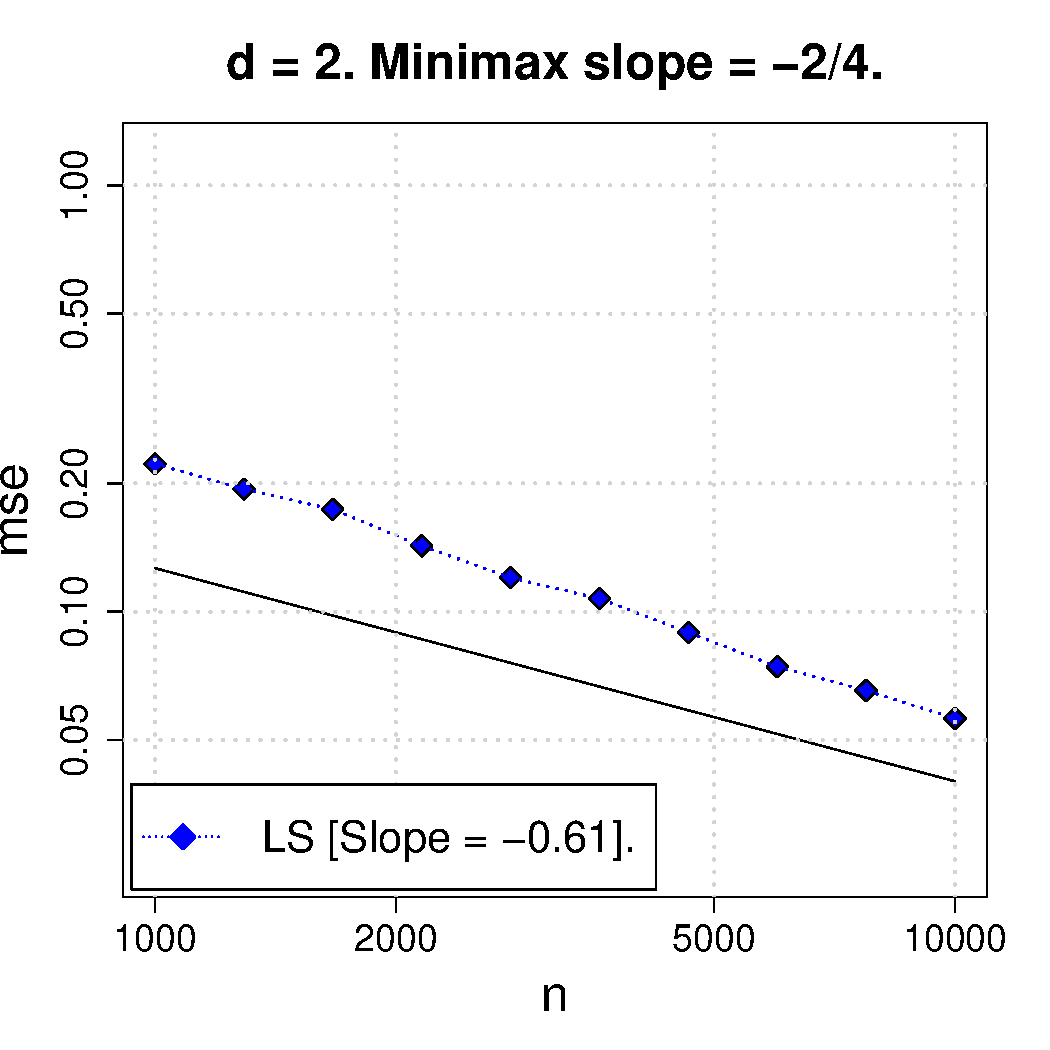
\includegraphics[width=.23\textwidth]{figures/cosine/mse_by_sample_size_2d.pdf}
	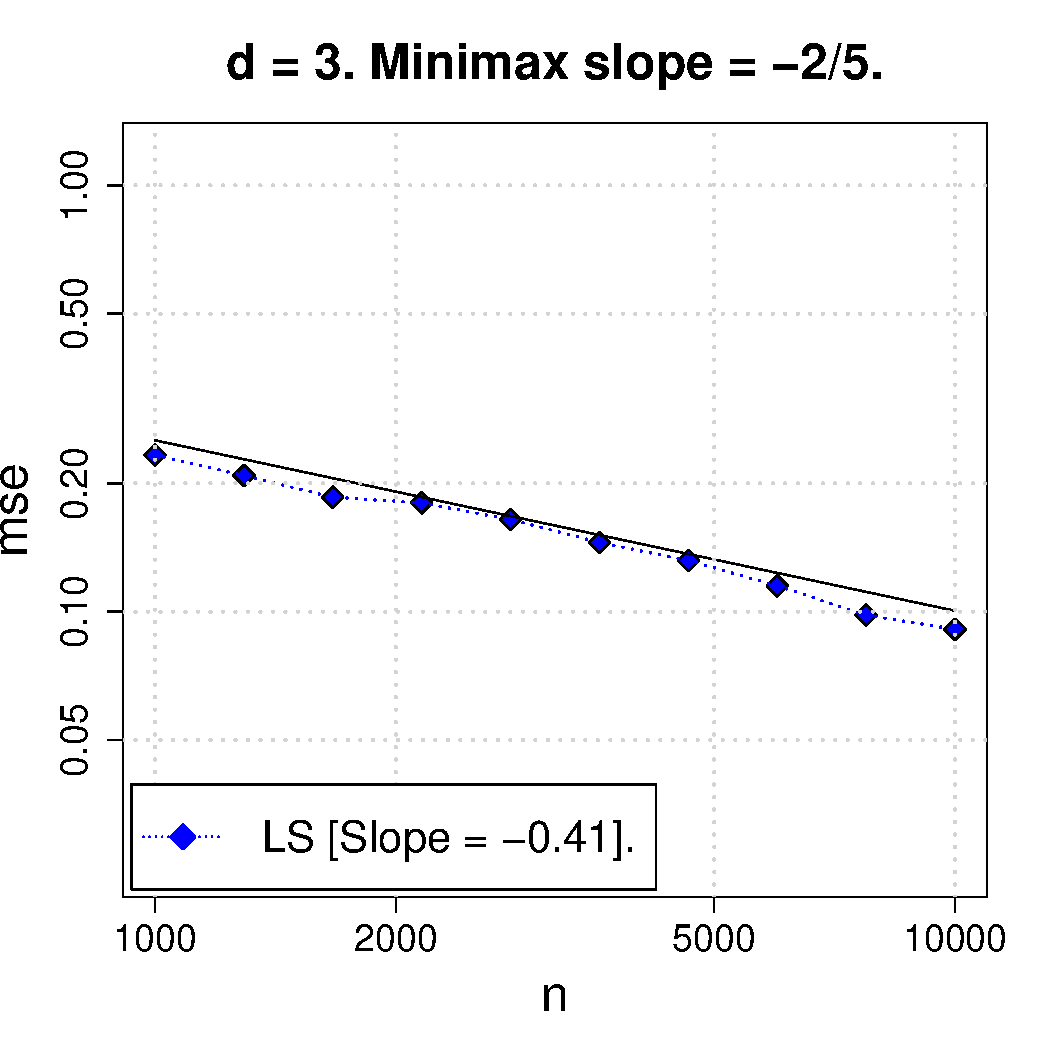
\includegraphics[width=.23\textwidth]{figures/cosine/mse_by_sample_size_3d.pdf}
	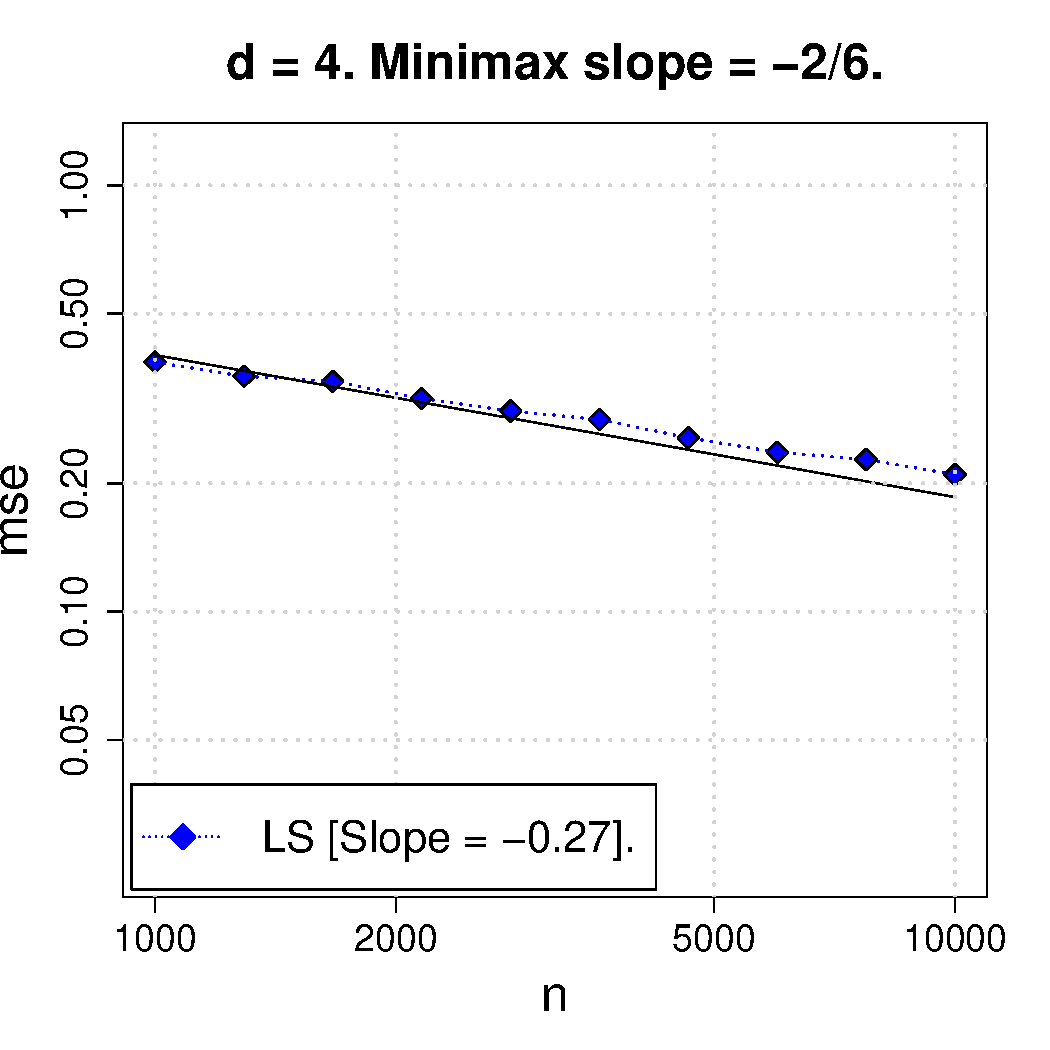
\includegraphics[width=.23\textwidth]{figures/cosine/mse_by_sample_size_4d.pdf}
	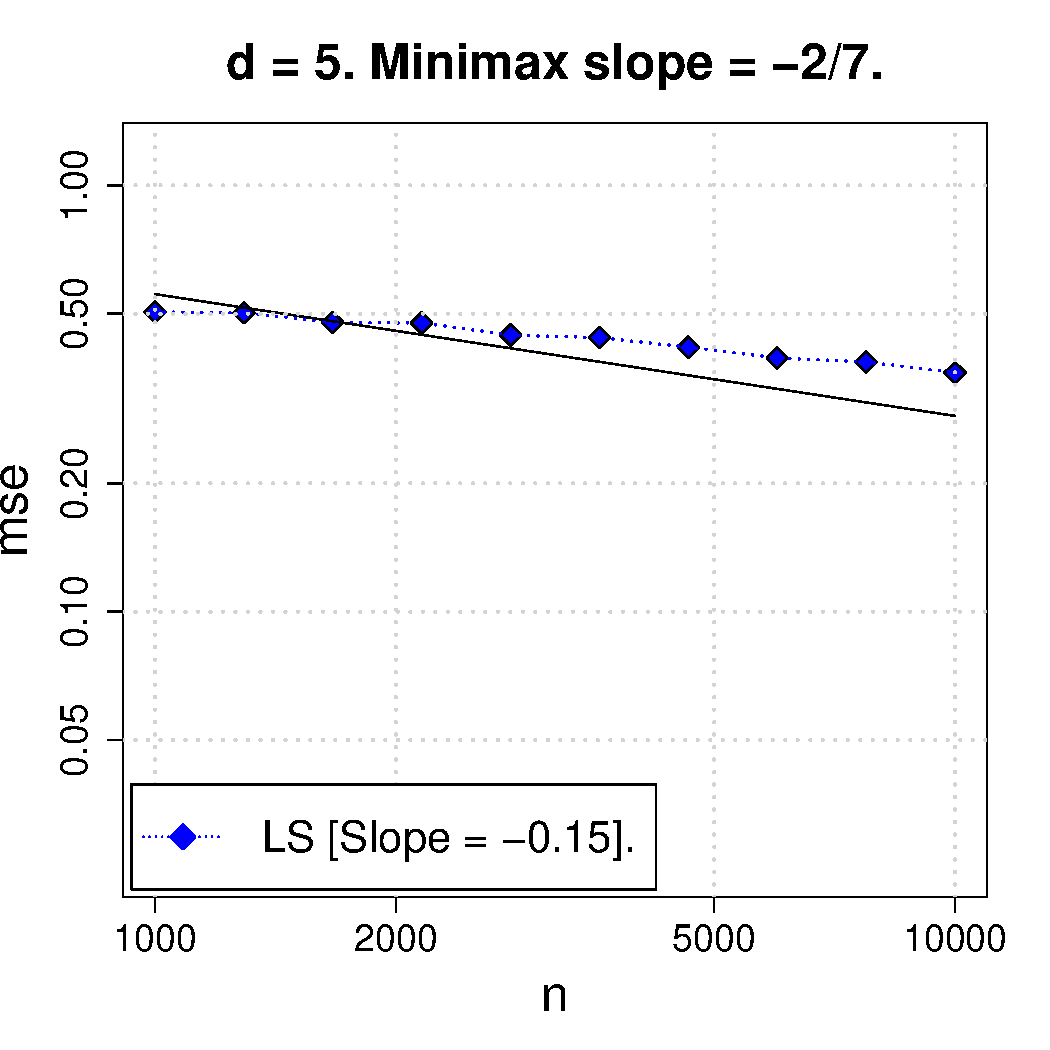
\includegraphics[width=.23\textwidth]{figures/cosine/mse_by_sample_size_5d.pdf}
	
	\caption{Comparison of Laplacian smoothing and $k$NN regression, as a function of sample size $n$. Plots are on the log-log scale, MSEs are averaged over 5 iterations, with both methods tuned for optimal MSE.  When $d = 1,2,3$, empirically both methods are achieving or exceeding the minimax rate.}
	\label{fig:fig1}
\end{figure}

\section{DISCUSSION}
\label{sec:discussion}

In this work, we have shown that Laplacian smoothing over a neighborhood graph is optimal, for various statistical problems and under various assumptions. 

There are still several extensions we feel are worth pursuing. In practice, it is more common to use $k$NN graphs than neighborhood graphs, due to the guaranteed connectivity and sparsity of the former; we strongly suspect that by building on the work of~\cite{calder2019}, one can show that our main results all hold when the $k$NN graph is used. In another direction, one can also generalize Laplacian smoothing by replacing the penalty $f^T \Lap_{n,r} f$ with $f^T \Lap_{n,r}^k f$ for some $k > 1$. The hope is that this adapted procedure would be minimax optimal over the previously mentioned higher-order Sobolev classes $H^k(\Xset)$. In the very special case of $k = 2$ and $d \leq 1 2$, we can show that this is indeed the case, but the general story--for all combinations of $k$ and $d$---remains beyond our reach. 

\bibliographystyle{plainnat}
\bibliography{../../../graph_testing_bibliography} 

\end{document}